\documentclass[12pt]{report}

% Font and text formatting packages
\usepackage{microtype} % Improved text alignment and spacing
\usepackage[bitstream-charter]{mathdesign}
\usepackage{XCharter} % XCharter font
\usepackage[scaled]{beramono} % Monospaced font styling
% \usepackage[italic]{mathastext} % Italicizes math in text font for consistency

% Conditional checking
\usepackage{etoolbox}

% Enhanced typography
\usepackage[normalem]{ulem} % Underlining
\usepackage{contour} % Outline text (used with \contour command)
\usepackage{xpatch} % Enables patching commmands for typographical modifications
\usepackage{bm} % Italic bold

% Scientific notation and chemical formulas
\usepackage[version=4]{mhchem} % For chemical notation
\usepackage{siunitx} % Consistent handling of units

% Graphics
\usepackage{graphicx} % Essential for including images
\usepackage{subcaption} % Subfigures and subcaptions
\graphicspath{{./images/}} % Path for images directory

% Document layout
\usepackage[margin=1in]{geometry} % 1-inch margins
\usepackage{multicol} % Multi-column layouts

% Custom captions formatting
\usepackage{caption}
\DeclareCaptionFormat{custom}{\textbf{#1.} #3}
\captionsetup{format=custom}


\usepackage{csquotes} % Recommended for quotes in citations
\usepackage[style=apa, backend=biber]{biblatex} % APA style citations
\addbibresource{references.bib} % Reference file


% Custom underlining with contour effect
\contourlength{1.7pt} % Default contour length
\NewDocumentCommand{\ul}{O{2.62pt} O{0.45pt} O{1.5pt} m}{%
  \begingroup%
  \renewcommand\ULdepth{#1}%
  \renewcommand\ULthickness{#2}%
  \contourlength{#3}%
  \uline{\phantom{#4}}\llap{\contour*{white}{#4}}%
  \endgroup%
}

% Additional custom commands
\def\code#1{\texttt{#1}} % Inline code styling
\newcommand{\goldenRatio}{1.6180} % Golden ratio constant
\newcommand{\inverseGoldenRatio}{0.6180} % Inverse golden ratio constant

% Define automatic kerning for footnotes next to punctuation
\makeatletter
\xpatchcmd{\@makefnmark}{\hss}{\kern-0.5em\hss}{}{}
\makeatother

% Automatic extra spacing around em-dashes
\xpretocmd{\textemdash}{\hspace{0.1em}}{}{}
\xapptocmd{\textemdash}{\hspace{0.1em}}{}{}

\title{\small{PHYS 461—Modern Physics Lab} \\ \huge{\textbf{Cavendish Experiment}} \\\vspace{-0.6cm}}
\date{
    \small{Report December 6, 2024 \\\vspace{0.05cm}
    Performed November 2024}
}
\author{
    \ul{Micah Hillman} \and Cordney Nash
}

\begin{document}\spacing{1.25}
\maketitle

\section*{Introduction}
{
    The Cavendish experiment, the namesake experiment of 18th century physicist Henry Cavendish, successfully measured the density of Earth, unintentionally allowing for the first measurement of Newton's universal gravitational constant \(G\)—calculated by later physicists~\cite{APS2008}. 
    The experiment uses a hermetically sealed torsion balance system to track the slow oscillation induced by bringing large masses (in our case, lead) in close proximity to a set of test masses connected to a torsional balance; by these means, the masses are made to interact gravitationally while minimizing the influence of extraneous forces~\cite{BMS2024}. 
    Bringing the test masses in close proximity changes the torsional pendulum's equilibrium position, to which the ensuing oscillations gradually decay (with a regular period—\(T\)—determined by the balance's moment of inertia and torsional constant)~\cite{BMS2024}. 
    By recording these oscillations and measuring the gravitationally-modulated torsional balance's changing equilibrium position, the universal gravitational constant \(G\) may be calculated~\cite{BMS2024}.
}

\section*{Theory}
{
At its core, the Cavendish experiment relies on forces described by Newtonian universal gravitation, famously expressed in the equation
    \begin{equation*}
        F_\mathrm{g} = G \frac{mM}{r^2}.
    \end{equation*} 
When large lead masses (\(M\)) are positioned in close proximity to the torsional balance's smaller masses (\(m\)), the equilibrium position of the torsional balance is suddenly altered, leading to slow \textit{oscillatory behavior} about a new equilibrium—the period (\( T \)) of which depends on the balance's torsional constant (\( \kappa \)) and moment of intertia (\( I = 2md^2 \)):
    \begin{equation}\label{period}
        T = 2\pi \sqrt{\frac{2md^2}{\kappa}}.
    \end{equation}
The torsional constant (\( \kappa \)) can be expressed as 
    \begin{equation}\label{torsion}
        \kappa = \frac{4GmMd}{r^2 \Delta \theta},
    \end{equation}
    so we can combine these two expressions (\ref{period},~\ref{torsion}) and isolate \(G\) in terms of observables and experimental parameters~\cite{BMS2024}:
        \begin{equation}
            G = \frac{2\pi^2r^2d\Delta\theta}{MT^2}. 
        \end{equation}


\section*{Methods}
{
    \begin{figure}[tbh]\centering
        \begin{subfigure}[t]{\linewidth}
          \centering
          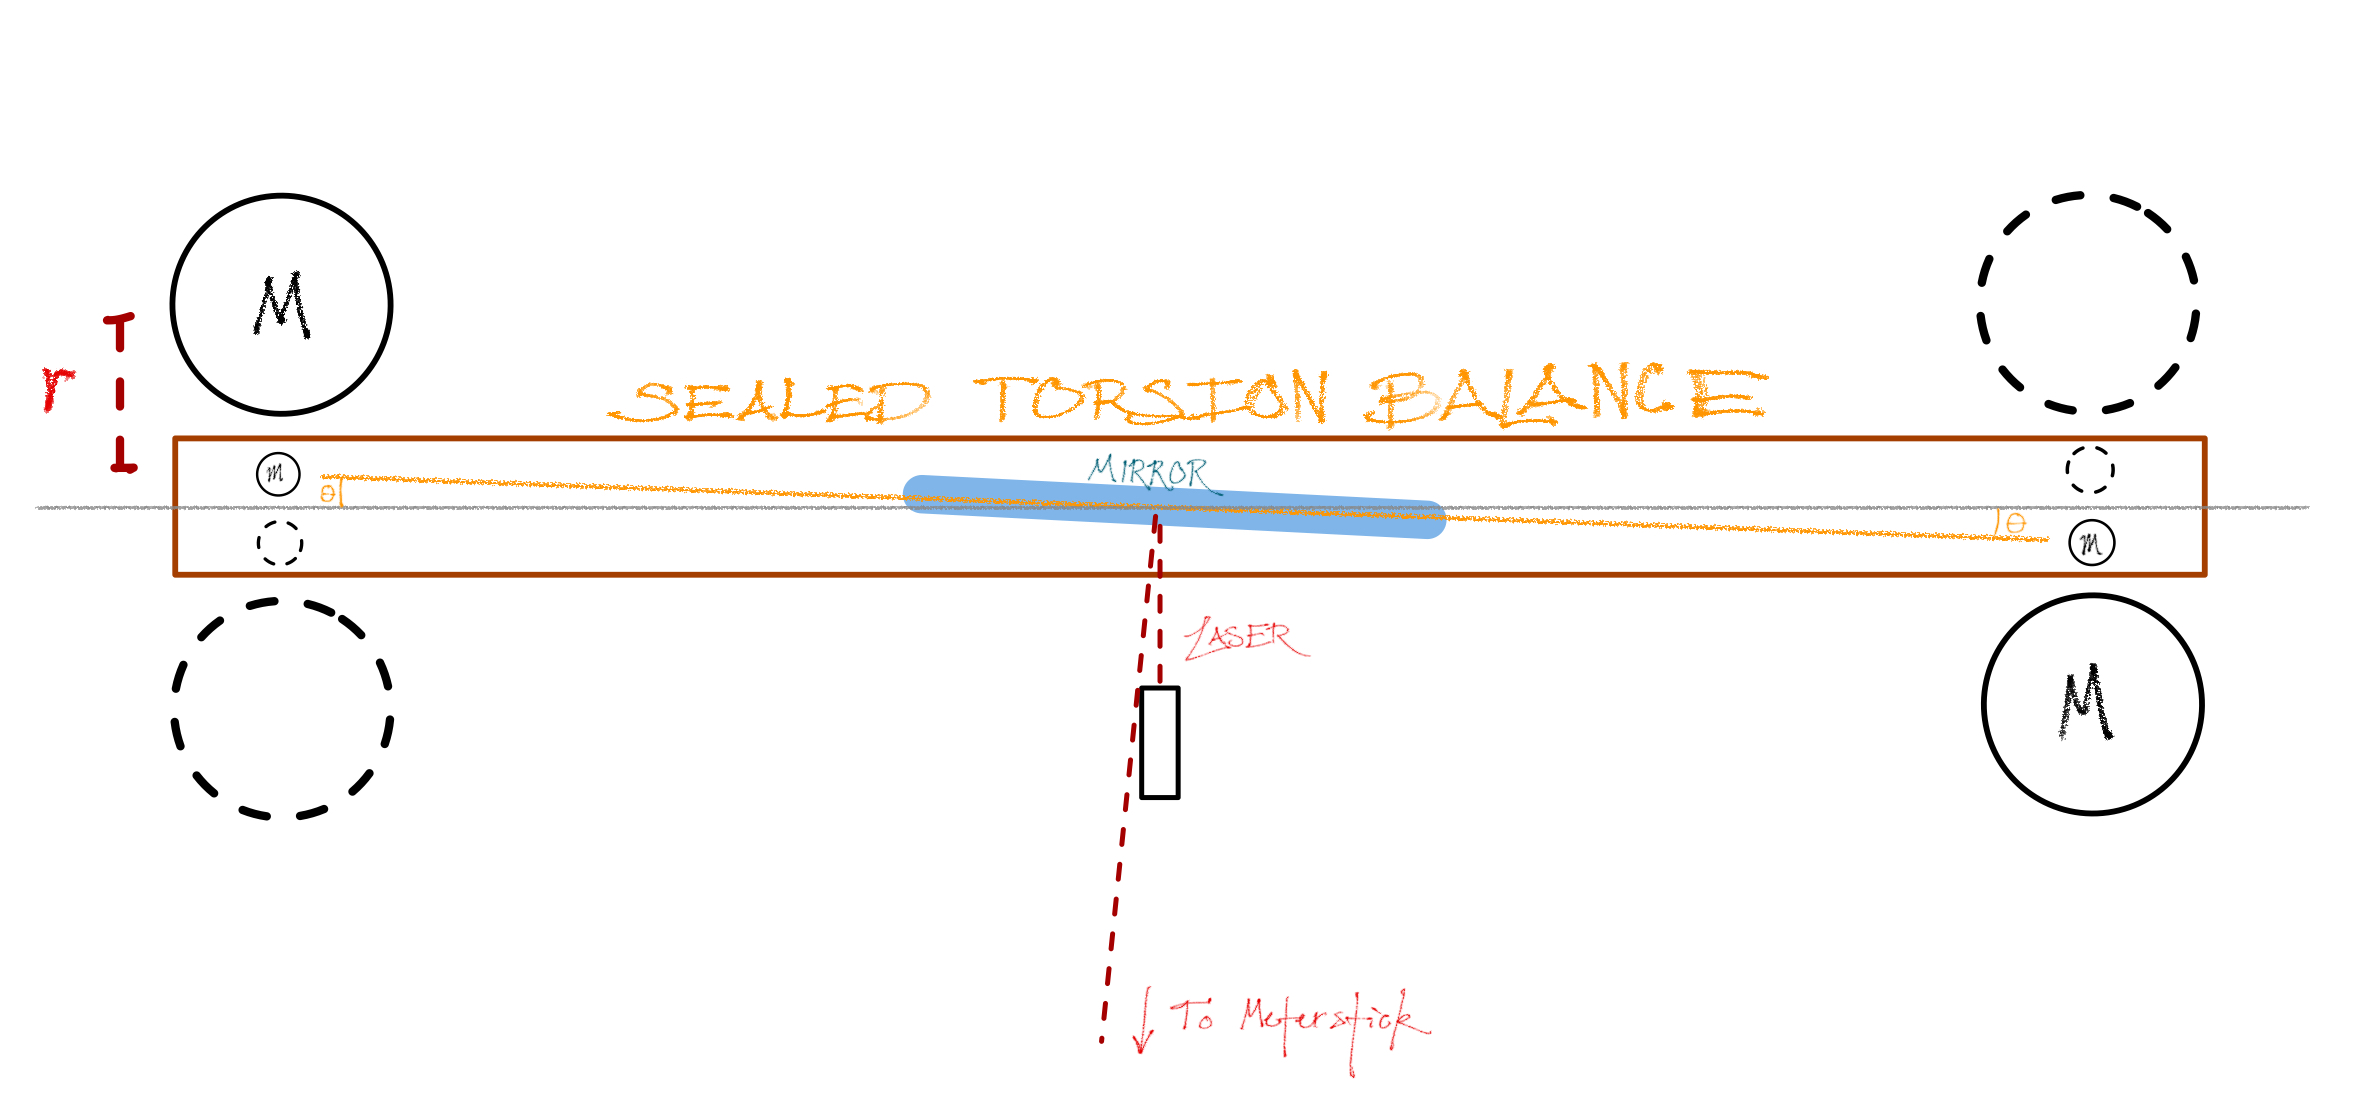
\includegraphics[width=\linewidth]{balance.jpeg}
          \caption{Birds-eye illustration of the sealed torsional balance system and associated weights. Important components include both the small and large lead masses \(m\) and \(M\), a reflective mirror attached to the central portion of the torsional balance beam, and a laser light which is reflected across the room to a measuring stick. }\label{balance}
        \end{subfigure}
        \vspace{1px} % Adjust vertical spacing as needed
        \begin{subfigure}[t]{\linewidth}
          \centering
          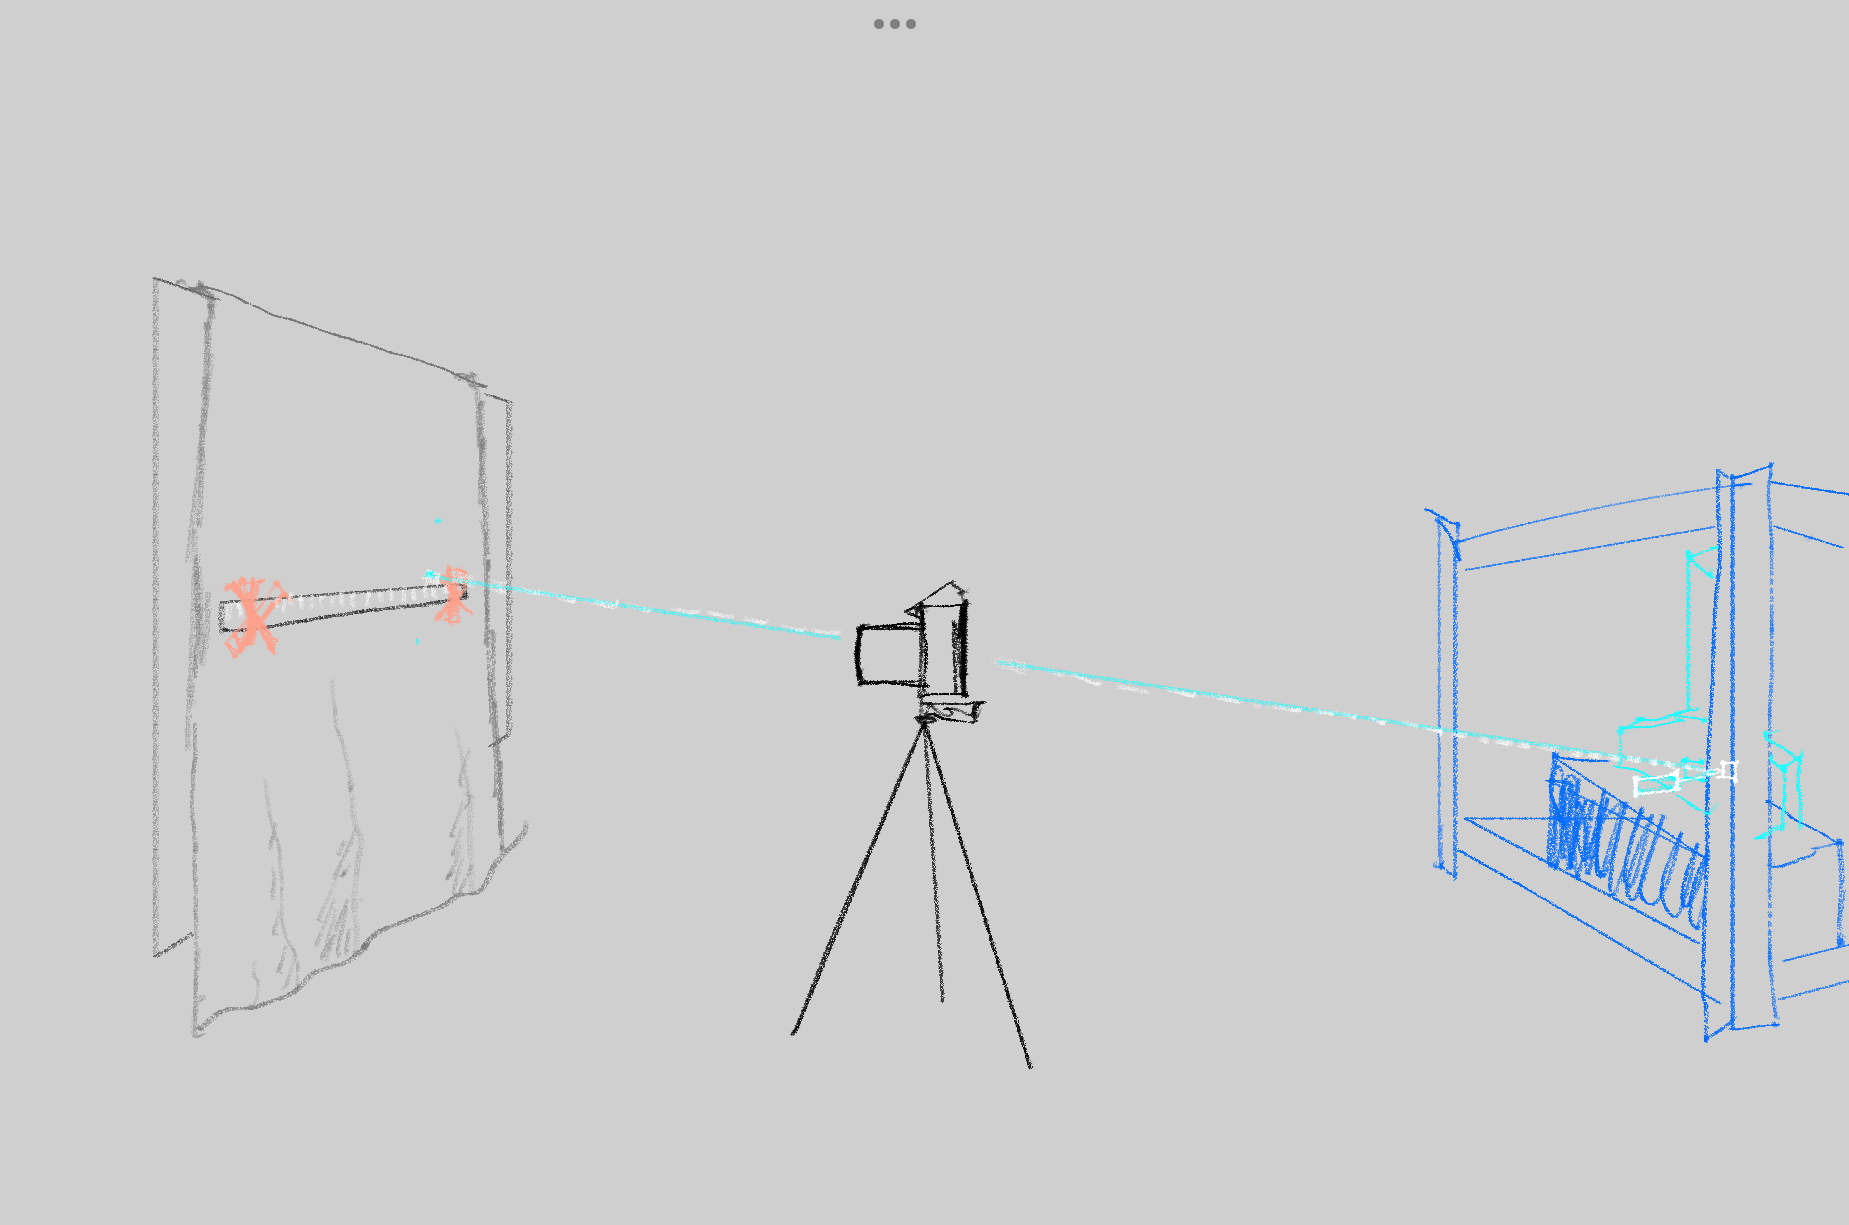
\includegraphics[width=\inverseGoldenRatio\linewidth]{board.jpeg}
          \caption{Illustration depicting measurement. A camera (center) and meter stick (left, at a known distance) were used to capture the positon of laser light reflected from the mirror affixed to central axis of the torsional balance (right, and shown in figure~\ref{balance}).}\label{board}
        \end{subfigure}
        \caption{Two sketched views of the Cavendish apparatus. Figure~\ref{balance} shows components associated with torsional balance system, while figure~\ref{board} depicts components associated with measurement.}
    \end{figure}



22kg lead sphere
}

\section*{Results}
{
    
}

\spacing{1.2}
\printbibliography{}

\end{document}